\documentclass{article}
%\usepackage{fullpage}
\usepackage{mathtools}
\usepackage{mhchem}
\usepackage{amssymb}
\usepackage{amsmath}
\usepackage{bm}
\usepackage{gensymb}
\usepackage{siunitx}
\usepackage{cancel}
\usepackage{graphicx}
\usepackage{subcaption}
\usepackage{mdframed}
\author{Mann, J}
\title{Day X Notes}
\date{MM DD, 2015}
\newenvironment{aside}{\begin{mdframed}}{\end{mdframed}}
\renewcommand{\d}[0]{\mathrm{d}}
\newcommand{\pOne}[2]{\frac{\partial #1}{\partial #2}}
\renewcommand{\deg}[0]{\degree}
\newcommand{\pTwo}[2]{\frac{\partial^2 #1}{\partial #2^2}}
\newcommand{\dOne}[2]{\frac{\d #1}{\d #2}}
\newcommand{\dTwo}[2]{\frac{\d^2 #1}{\d #2^2}}
\newcommand{\diag}[1]{\bcancel{#1}}
\newcommand{\matr}[1]{\bm{#1}}
\newcommand{\note}[1]{\vspace{3\parsep}\textit{\textbf{Note: }}#1\vspace{2\parsep}}
\newcommand{\norm}[1]{\left|#1\right|}
\newcommand{\aone}[0]{\vec{a}_1}
\newcommand{\atwo}[0]{\vec{a}_2}
\newcommand{\bone}[0]{\vec{b}_1}
\newcommand{\btwo}[0]{\vec{b}_2}
\newcommand{\pmat}[1]{\begin{pmatrix}#1\end{pmatrix}}
\newcommand{\nhat}[0]{\hat{n}}
\newcommand{\nvec}[0]{\vec{n}}

\graphicspath{{Day13NotesPics/}}
\begin{document}
\maketitle{}
\begin{section}{Intro}
	\begin{itemize}
		\item Notations for surface adrobent, adsorbate pairs.
		\item Catalysis comments
	\end{itemize}
	Later in the lecture\dots
\end{section}
\begin{section}{Structure}
	\begin{enumerate}
		\item 	Translational symmetry
			You saw translational symmetry in the image of platinum on a carbon backing. Translational symmetry was only true in certain domains.

		\item Rotational symmetry
			You can rotate it using the $\matr{Q}$ matrix I showed you last time,
			\begin{align*}
				\matr{Q} = \pmat{\cos\theta & -\sin\theta\\\sin\theta & \cos\theta}
			\end{align*}

			Thre are 5 meshes that have these two symmetries (in two dimensions).
			What are they?
			Primitive square
			\begin{figure}[h]
				\centering
				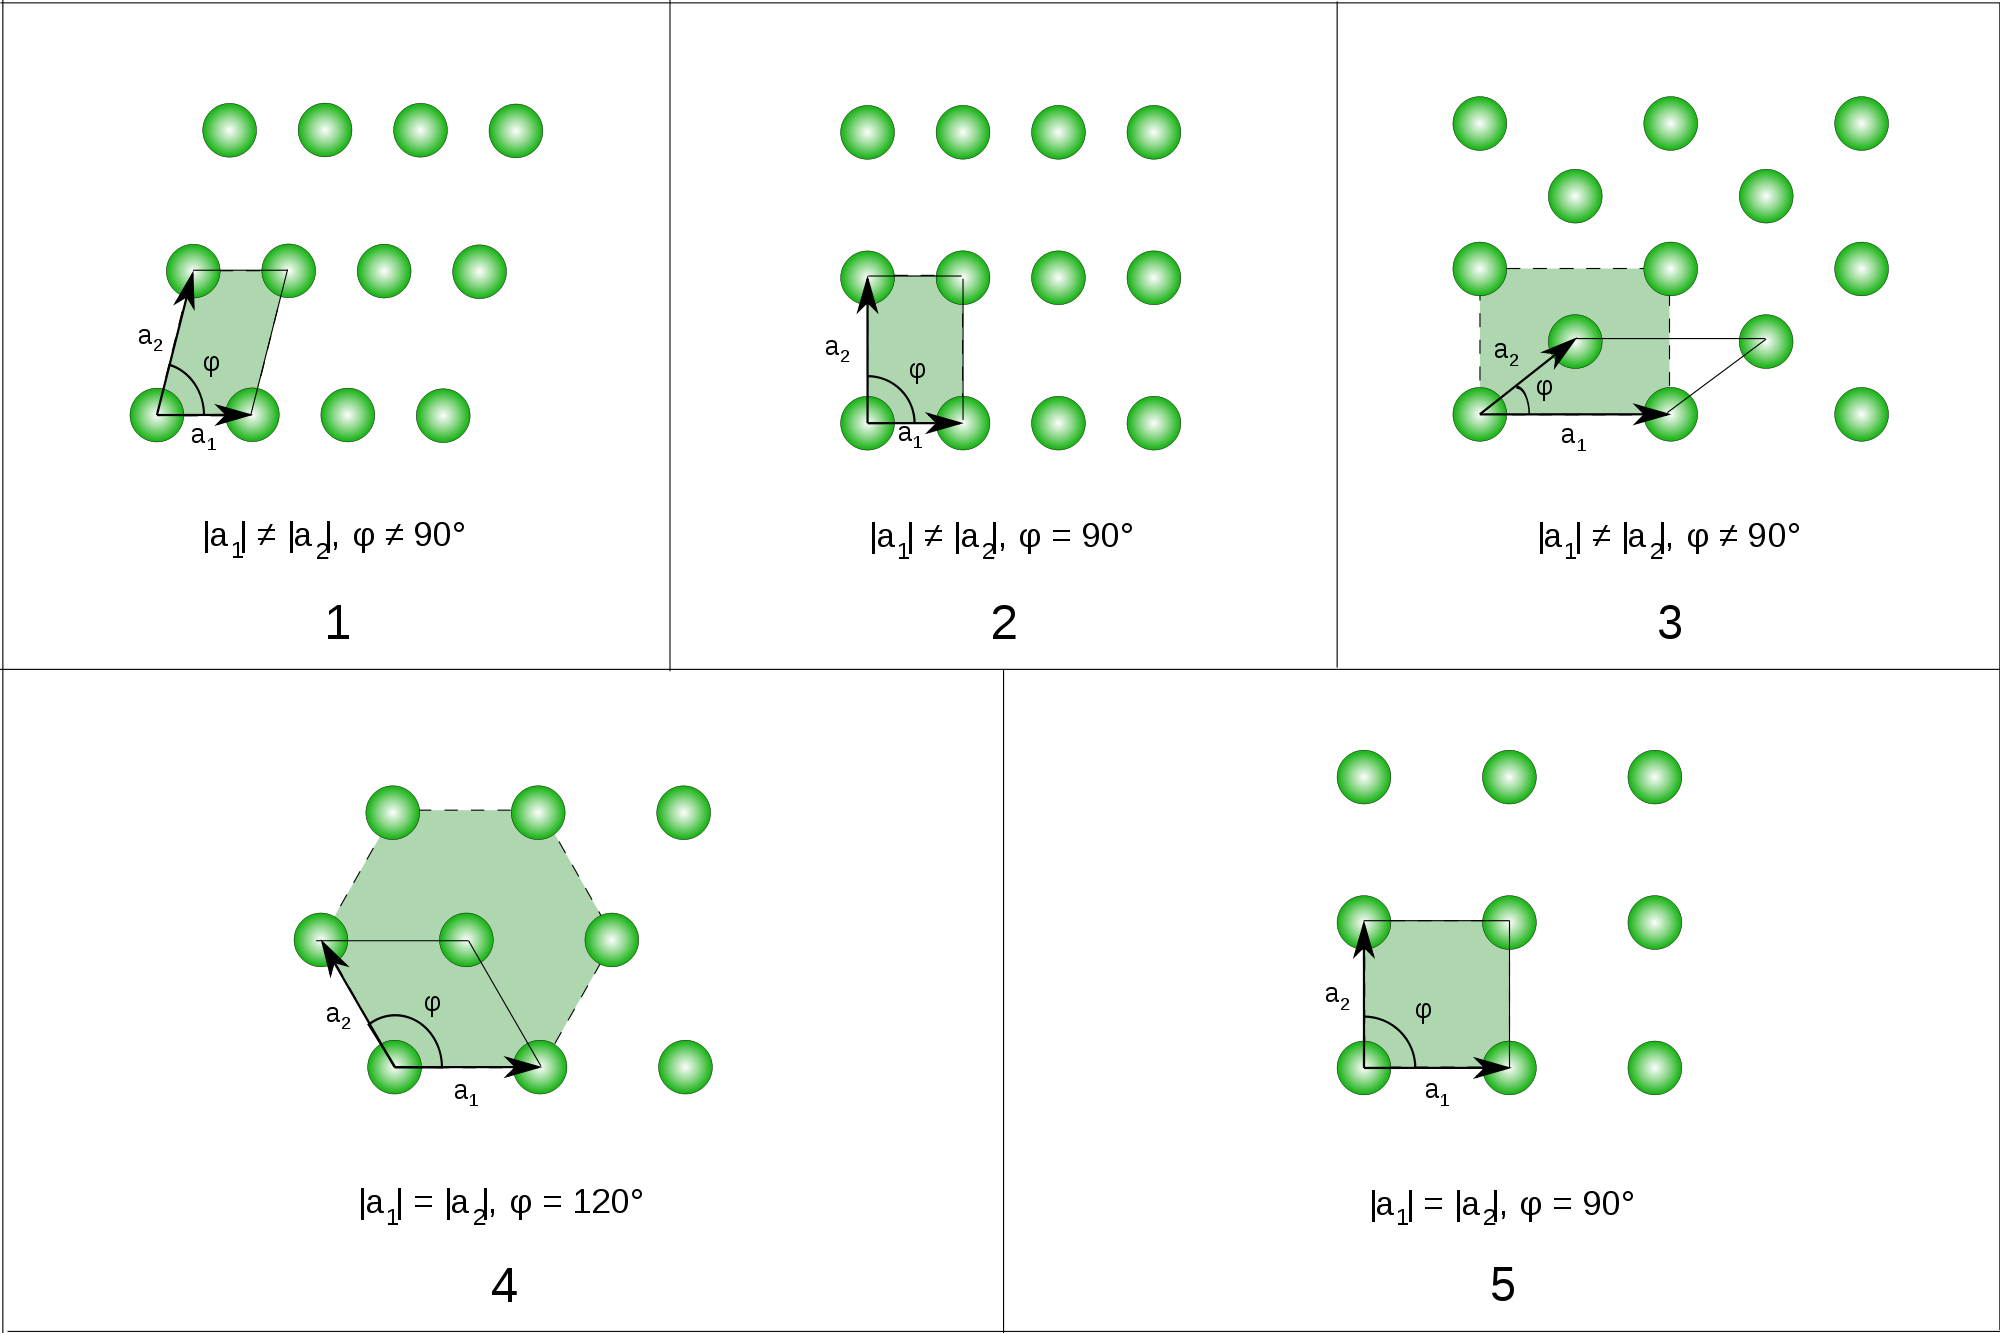
\includegraphics[height=160pt]{bravaislattices}
				\caption{Here are the bravais lattices in two dimensions}
				\label{fig:bravais}
			\end{figure}

			\begin{itemize}
				\item Square
					\begin{align*}
						\norm{\aone} = \norm{\atwo}
					\end{align*}
					Angles are $90^\circ$.


				\item Second Primitive rectangle
					\begin{align*}
						\norm{\aone} \neq\norm{\atwo}
					\end{align*}
					Angles are $90^\circ$
					Rectangle

				\item Centered rectangle.

					\note{Not a square centered lattice. This is not necessary}


				\item Oblique
					\begin{align*}
						\norm{\aone}\neq\norm{\atwo}
					\end{align*}
					Angles $\neq 90^\circ$

				\item Hexagonal/Triangular Net
					\begin{align*}
						\norm{\aone}\neq\norm{\atwo}
					\end{align*}
					angle is $120^\circ$
			\end{itemize}
	\end{enumerate}

	If you assent translational and rotational symmetry, then you can rotate 
	\begin{align*}
		\begin{matrix}\frac{2\pi}{1} & \frac{2\pi}{2} & \frac{2\pi}{3} & \frac{2\pi}{4} & \frac{2\pi}{6}\\
			360/0^\circ & 180^\circ & 120^\circ & 90^\circ & 60^\circ\end{matrix}
	\end{align*}
	\note{The $\frac{2\pi}{5}$ is excluded, which is an icosahedral, may exist}


	With large crystal faces, it would be very unusual to find an icosahedral.


\end{section}
\begin{section}{Wood's Notation}
	The most common notation is by one Elizabeth Wood.
	\begin{align*}
		R(hkl)\pmat{P\\\text{or}\\ C}\frac{\norm{\bone}}{\norm{\aone}}\times \frac{\norm{\btwo}}{\norm{\atwo}} - \alpha - D
	\end{align*}
Where $\alpha$ is the angle, and $D$ is the adsorbate symbol.
	$hkl\Rightarrow$ location of substrate

	The two vectors $\bone$ and $\btwo$ have the same angle as $\aone$ and $\atwo$. You may need to rotate the vectors $\aone$ and $\atwo$ relative to $\bone$ and $\btwo$ to get the location of the add vector.

	There is really only one problem for the Elizabeth Wood formulation:

	Not always are these two angles equal.  

	So there is a more general notation.
\end{section}
\begin{section}{More Generally}
	\begin{align*}
		R(hkl)\pmat{P\\\text{or}\\ C} - \matr{G} - D
	\end{align*}
	\begin{align*}
		\matr{B}=\pmat{\bone\\\btwo}
		\matr{A}=\pmat{\aone\\\atwo}
		\matr{B}=\matr{G}\cdot\matr{A}\\
		\matr{G}=\matr{B}\cdot\matr{A}^{-1}
	\end{align*}

	Once you know $R(hkl)$ lattice plane, and you know $P$ or $C$, then $\matr{G}$ tells the tale of where $D$ is located.

\begin{subsection}{One other point that comes up}
	The determinant of $\matr{G}$ has additional information that is on it (nice properties).

	The question that you want to ask is whether $\det{\matr{G}}$ is a rational number or not. ($\matr{G} = P \in \mathbb{I^+} - {0}$)  If so, the overlayer and substrate are rationally organized.

	If $\det{\matr{G}} = \frac{P}{q}, P,q \in \mathbb{I^+} - {0}$, the nets are said to be rationally related. Otherwise the two nets are said to be irrational, which means that there is not a 
	rational way to superimpose the adsorbate net on the adsorbent.

	If the structures are rational, then a coincident net exists. i.e. $\det{\matr{G}}=\frac{P}{q}$, then you can find a net 
	\begin{align*}
		\pmat{\vec{C}_1\\\vec{C}_2} = \matr{P}\pmat{\aone\\\atwo}\\
		\pmat{\vec{C}_1\\\vec{C}_2} = \matr{Q}\pmat{\bone\\\btwo}
	\end{align*}
	Where $\matr{Q}$ is \underline{not} the rotation matrix. If the nets are coincident, the authors may only give you $\vec{C}_1$ and $\vec{C}_2$. 

\end{subsection}

Suppose you have a catalytic surface (Ni(111) for example). The first thing you want to do is to remind yourself which surface is the (111) surface. Then you can unfold that surface and there is the unit net

\begin{figure}[h]
	\centering
	%\includegraphics[height=100pt]{111net}
	\caption{The 111 surface with the unit net on it}
	\label{fig:111net}
\end{figure}
Now you have a plane, and a normal. You can find 

$\aone\times\atwo = \nhat$.

The domain, $D$ is arbitrary for now. Now if I overlay \ce{CO}

$\ce{Ni}(111)(2\times 2)$

\begin{figure}[h]
	\centering
	%\includegraphics{surfacePic}
	\caption{111 surface of Nickel}
	\label{fig:111surf}
\end{figure}

\begin{align*}
	\dOne{}{t}\int_{D}\Gamma(x,y,t)\d A &= - \oint_{\partial D}\hat{m}\cdot \vec{J}^s\d S - \int_{A}\nhat\cdot \vec{J}^{(+)}\d A
\end{align*}
Where $J^{(+)}$ is the flux from the vapor side down onto the surface, at the surface. $J^s$ is the flux across the surface.
\end{section}
\end{document}
